
\chapter{Detection networks}
\label{sec:detnets}
The goal of the detection network is to localize all objects of chosen categories. There is a simple logical step from classification to detection. It is to classify selected regions in the image as one of the classes or as a background. A classification applied to every possible box in the image would undoubtedly produce great detection results but at the extreme computational cost. This section describes a family of algorithms based on this simple idea while managing limited computational resources.

We will see that this family of so-called \textit{region based} approaches can reach state-of-the-art results, with increasing efficiency by each generation. Considering precision, Faster R-CNN is still used as one of the most reliable detectors. However, although it can process a few frames per second, we do not consider it to be a truly real-time detector and applicable for demanding tasks, such as video surveillance. We devote \cref{sec:rltm} to detection networks performing in real-time constraints.

\section{R-CNN (2014)}
Region-based Convolutional Network (R-CNN) by \citeauthor{bib:rcnn} \cite{bib:rcnn} is the first member of the family of region-based detection models. The foundation idea is simple: select regions in the picture and classify each region. This approach leads to a combination of three modules: region proposal algorithm, feature extraction using CNNs on those regions and subsequent classification. 

A naive approach would use a sliding window and classify each cutout of the image. However, examining all the windows for different sizes and aspect ratios of possible objects would be extremely slow. R-CNN solves this problem by applying a region proposal algorithm that selects about 2000 most likely locations of objects. Regions are selected using the \textit{Selective search} (SS) \cite{bib:selectivesearch} algorithm and serve as a candidates for bbox predictions. In addition, bounding box regression can be trained to improve bbox prediction accuracy.

Each region is processed separately by a CNN into a feature map (the original architecture uses Alexnet, but any classification network can be substituted). Finally, each feature map can be scored. R-CNN uses class specific linear support-vector machines instead of a soft-max classification provided by CNNs. \Cref{fig:rcnn} illustrates the architecture.

\begin{figure}
    \centering
    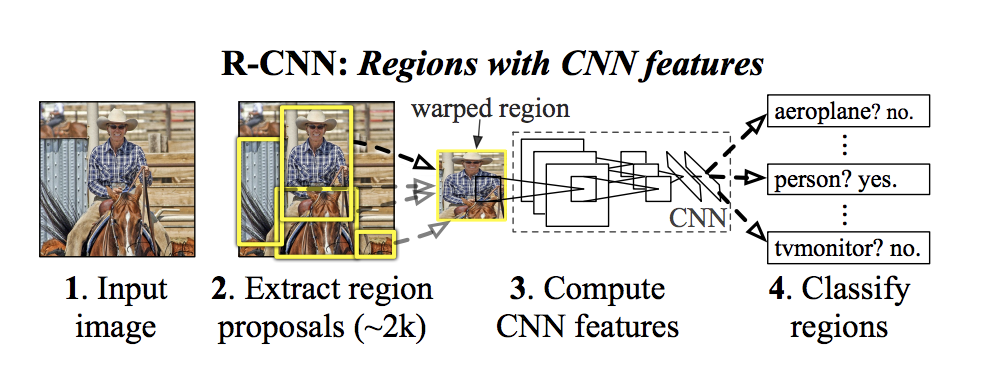
\includegraphics[width=\textwidth]{img/rcnn}
    \caption[R-CNN architecture]%
    {R-CNN architecture. Taken from \cite[fig. 1]{bib:rcnn}.}
    \label{fig:rcnn}
\end{figure}

\section{Fast R-CNN (2015)}
Even though R-CNN was a major step in the right direction, its performance is far from real-time. \citeauthor{bib:fastrcnn} \cite{bib:fastrcnn} introduces Fast R-CNN with a series of innovations to its predecessor, aimed at improving speed and accuracy. Provided benchmark on the NVIDIA K40 GPU suggests improvements from 47 seconds per image using R-CNN with VGG16 feature extractor, to 320 milliseconds with Fast R-CNN using the same feature extractor (not including time for SS proposals). 

Similarly to R-CNN, this architecture also utilizes region proposal algorithm and a CNN to produce a feature map. A significant drawback of R-CNN was computing feature map for each region, despite overlaps. Fast R-CNN processes whole input image into a feature map, and then, using a \textit{region of interest (RoI) pooling layers}, extracts a feature vector for each region. All extracted feature vectors are pooled to the same size and are passed through a series of fully connected layers, leading to softmax classifier and bounding box regression layer. An illustration of this process can be seen on \cref{fig:fastrcnn}.

\begin{figure}
    \centering
    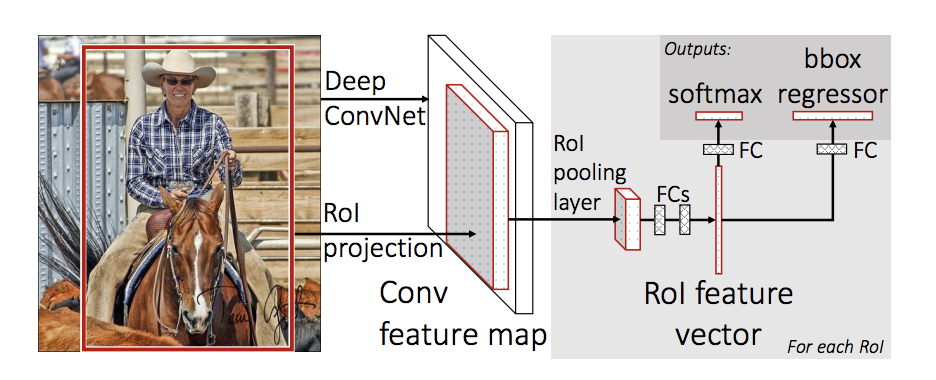
\includegraphics[width=\textwidth]{img/fastrcnn}
    \caption[Fast R-CNN architecture]%
    {Fast R-CNN architecture. Taken from \cite[fig. 1]{bib:fastrcnn}}
    \label{fig:fastrcnn}
\end{figure}

\section{Faster R-CNN (2015)}
 
Faster R-CNN by \citeauthor{bib:fasterrcnn} \cite{bib:fasterrcnn} expands on the Fast R-CNN with the aspiration to achieve real-time performance. Fast R-CNN managed to build a fast feature extraction and subsequent classification usable in a real-time environment. However, it is heavily slowed down by a region proposal SS algorithm. Faster R-CNN expands on the idea of sharing resources and replaces SS with \textit{region proposal network} (RPN). RPN is built on top of a feature map generated by the feature extractor. As suggested, the feature map is shared between RPN and object detection. This approach is able to achieve 5 fps, which can find limited use in a real-time environment. Whole architecture can be seen on \cref{fig:fasterrcnn}. 
 
 \paragraph{Region proposal network} is designed as a small, sliding-window network, with negligible cost compared to the feature extractor. It is composed of 3$\times$3 convolutional layer with 512 filters and two sibling 1$\times$1 convolutional layers for region regression and classification. Classification in RPNs determines whether proposed region contains an object or a background (\textit{cls} score). Region regression part of the network is tied to the concept of \textit{anchors} (the anchor is a predefined box centered at a location of sliding-window). Assuming \textit{k} anchors with different sizes and aspect ratios are used, regression produces 4k relative parameters and classifier 2k scores. Regression parameters are used to modify the position and size of their corresponding anchor. The number of regions is then reduced by eliminating proposals with high overlap using a \textit{non-maximum suppression} (NMS) based on \textit{cls} score. After NMS, top-N ranked proposal regions are used for detection.
 
 To calculate loss and train RPN, a matching between ground-truth boxes and generated region proposals needs to be determined. A positive label is assigned to two kinds of regions: the one with the highest IoU overlap with ground-truth box; regions that have IoU higher than 0.7 with any ground-truth box. A negative label is assigned to a non-positive box if its IoU is lower than 0.3 for all ground-truth boxes. Rest of the boxes do not contribute to training. 
 
 \paragraph{4-step alternating training:}
 
 \begin{enumerate}
     \item train RPN with feature extractor initialized by ImageNet pre-trained model
     \item train separate Fast R-CNN using proposals generated by RPN from step 1
     \item train RPN with feature extractor initialized by weights learned by the detector in step 2, fine-tune only layers unique to RPN
     \item using the model from step 3, fine-tune layers unique to Fast R-CNN
 \end{enumerate}

\noindent Thanks to the modular architecture, R-CNN family networks can exploit any CNN as a feature extractor.  Therefore Faster R-CNN can achieve state-of-the-art detection results exploiting the latest advances in classification networks and is often used as a benchmark of their performance.
     

 \begin{figure}
     \centering
     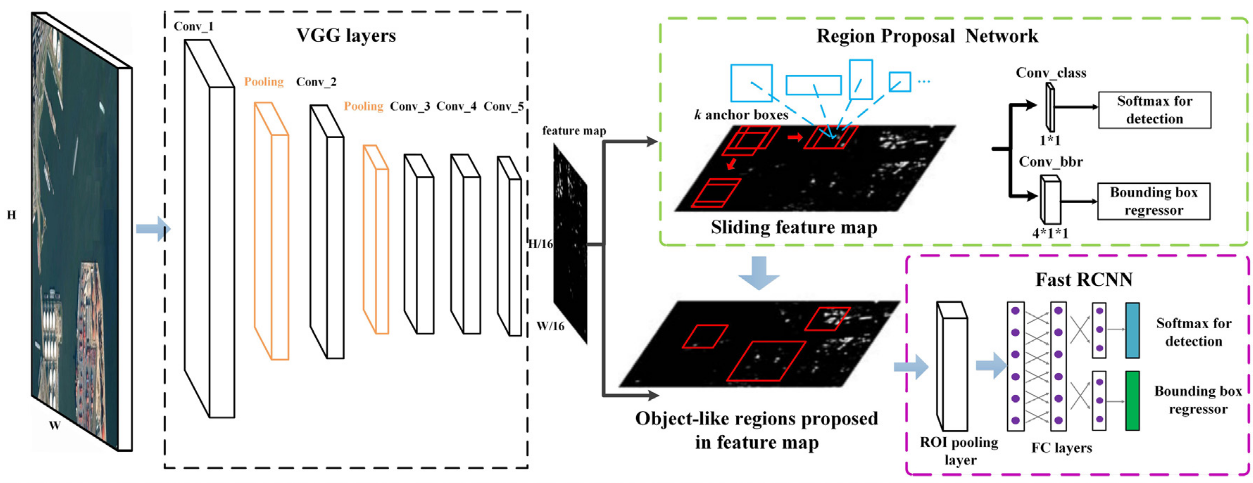
\includegraphics[width=\textwidth]{img/fasterrcnn}
     \caption[Faster R-CNN architecture]%
     {The architecture of Faster R-CNN. From \url{https://researchgate.net/figure/The-architecture-of-Faster-R-CNN\_fig2\_324903264}.}
     \label{fig:fasterrcnn}
 \end{figure}

\section{Mask R-CNN (2017)}
Previous R-CNN based architectures used bounding boxes to localize individual objects. \citeauthor{bib:maskrcnn} \cite{bib:maskrcnn} adds a localization based on semantic segmentation, where the goal is to classify each pixel into a category. 

Mask R-CNN is built upon Faster R-CNN and combines both bounding box localization and semantic segmentation by predicting segmentation masks for each RoI. The product of this approach is a bounding box and class for each object, together with a binary segmentation mask. Unlike the semantic segmentation on whole input, applying it on RoIs allows for \textit{instantiated segmentation} where selected pixels corresponds to a given instance of a class.

Implementation and architecture are very similar to Faster R-CNN, with two exceptions. One of them is already described, fully convolutional segmentation branch which works in parallel with classification and bounding box regression heads. The other difference is a replacement of RoI pooling layer with \textit{RoI alignment layer}. The problem of RoI pooling for this purpose is quantization of floating-number RoI to discrete feature map grid and consequent imprecision. RoI alignment mitigates this problem by using bi-linear interpolation to compute exact values of features at four sampled location in each of RoIs locations and aggregating the results. High-level architecture and the RoI alignment layer are visualized on \cref{fig:maskrcnn}.

 \begin{figure}
     \centering
     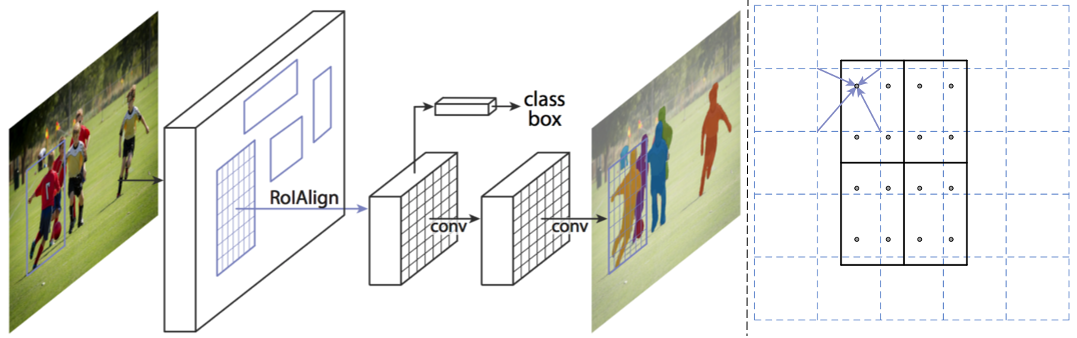
\includegraphics[width=\textwidth]{img/maskrcnn}
     \caption[Mask R-CNN architecture and RoI alignment layer]%
     {Left: The architecture of Mask R-CNN. Right: RoI align, grid represents feature map, solid lines an RoI and the dost are the sampling points. From \cite[fig. 1, 3]{bib:maskrcnn}}
     \label{fig:maskrcnn}
 \end{figure}

